% mnras_template.tex 
%
% LaTeX template for creating an MNRAS paper
%
% v3.0 released 14 May 2015
% (version numbers match those of mnras.cls)
%
% Copyright (C) Royal Astronomical Society 2015
% Authors:
% Keith T. Smith (Royal Astronomical Society)

% Change log
%
% v3.0 May 2015
%    Renamed to match the new package name
%    Version number matches mnras.cls
%    A few minor tweaks to wording
% v1.0 September 2013
%    Beta testing only - never publicly released
%    First version: a simple (ish) template for creating an MNRAS paper

%%%%%%%%%%%%%%%%%%%%%%%%%%%%%%%%%%%%%%%%%%%%%%%%%%
% Basic setup. Most papers should leave these options alone.
\documentclass[fleqn,usenatbib]{mnras}

% MNRAS is set in Times font. If you don't have this installed (most LaTeX
% installations will be fine) or prefer the old Computer Modern fonts, comment
% out the following line
\usepackage{newtxtext,newtxmath}
% Depending on your LaTeX fonts installation, you might get better results with one of these:
%\usepackage{mathptmx}
%\usepackage{txfonts}

% Use vector fonts, so it zooms properly in on-screen viewing software
% Don't change these lines unless you know what you are doing
\usepackage[T1]{fontenc}
\usepackage{ae,aecompl}


%%%%% AUTHORS - PLACE YOUR OWN PACKAGES HERE %%%%%

% Only include extra packages if you really need them. Common packages are:
\usepackage{graphicx}	% Including figure files
\usepackage{amsmath}	% Advanced maths commands
\usepackage{amssymb}	% Extra maths symbols

%%%%%%%%%%%%%%%%%%%%%%%%%%%%%%%%%%%%%%%%%%%%%%%%%%

%%%%% AUTHORS - PLACE YOUR OWN COMMANDS HERE %%%%%

% Please keep new commands to a minimum, and use \newcommand not \def to avoid
% overwriting existing commands. Example:
%\newcommand{\pcm}{\,cm$^{-2}$}	% per cm-squared

\usepackage{verbatim}   % added by JP for the TC word count output.

%%%%%%%%%%%%%%%%%%%%%%%%%%%%%%%%%%%%%%%%%%%%%%%%%%

%%%%%%%%%%%%%%%%%%% TITLE PAGE %%%%%%%%%%%%%%%%%%%

% Title of the paper, and the short title which is used in the headers.
% Keep the title short and informative.
\title[Radon trace profiles of PSB galaxies]{Radon transform trace profiles of PSB galaxy stellar velocity fields}

% The list of authors, and the short list which is used in the headers.
% If you need two or more lines of authors, add an extra line using \newauthor
\author[John Proctor]{
John Proctor$^{1,2}$\thanks{E-mail: jp210@st-andrews.ac.uk (JP)}
% A. N. Other,$^{2}$
% Third Author$^{2,3}$
% and Fourth Author$^{3}$
\\
% List of institutions
$^{1}$Royal Astronomical Society, Burlington House, Piccadilly, London W1J 0BQ, UK\\
$^{2}$School of Physics and Astronomy, University of St Andrews, North Haugh, St Andrews KY16 9SS, UK\\
}


% These dates will be filled out by the publisher
\date{Accepted XXX. Received YYY; in original form ZZZ}

% Enter the current year, for the copyright statements etc.
\pubyear{2019}

% Don't change these lines
\begin{document}
\label{firstpage}
\pagerange{\pageref{firstpage}--\pageref{lastpage}}
\maketitle

% Abstract of the paper
\begin{abstract}
A short document to present and discuss Radon trace profiles of stellar velocity maps for a sample of 30 central-type post-starburst galaxies. 
\end{abstract}

% Select between one and six entries from the list of approved keywords.
% Don't make up new ones.
\begin{keywords}
keyword1 -- keyword2 -- keyword3
\end{keywords}

%%%%%%%%%%%%%%%%% BODY OF PAPER %%%%%%%%%%%%%%%%%%

\section{Introduction}

\citet{2018MNRAS.480.2217S} utilise the Radon transform of MaNGA-derived velocity field maps to detect asymmetries and disturbances in the velocity fields of galaxies as obtained from the SDSS-IV MaNGA survey. Here we examine the Radon transform trace profiles of a sample of 30 central-type post-starburst (CPSB) galaxies and compare these Radon profile trace plots with those of a corresponding control sample of non-CPSB, or 'normal' galaxies.

\subsection{Radon trace profiles of CPSBs}

The Radon transform trace profiles of the CPSB sample are presented in Figures \ref{fig:Radon-traces-CPSBs-1} and \ref{fig:Radon-traces-CPSBs-2}. We subdivide the CPSB sample the trace plots across two figures in order to display these clearly on the page. There is no other significance in the split over Figures \ref{fig:Radon-traces-CPSBs-1} and \ref{fig:Radon-traces-CPSBs-2}.

\begin{figure*}
    \centering
    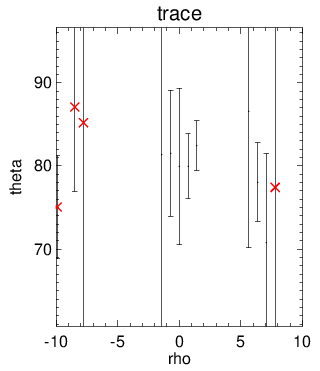
\includegraphics[width=0.23\textwidth]{Images/trace-plots/trace-plots-cpsbs/7964-1902.png}
    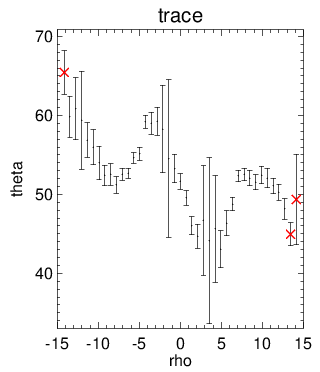
\includegraphics[width=0.23\textwidth]{Images/trace-plots/trace-plots-cpsbs/8080-3702.png}
    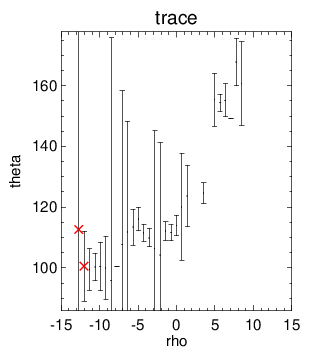
\includegraphics[width=0.23\textwidth]{Images/trace-plots/trace-plots-cpsbs/8081-3702.png}
    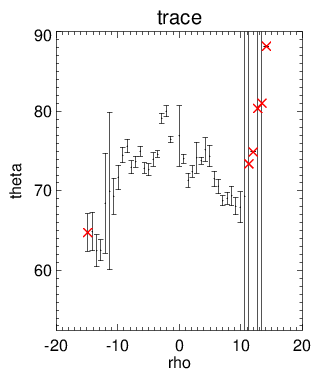
\includegraphics[width=0.23\textwidth]{Images/trace-plots/trace-plots-cpsbs/8082-3704.png}
    %
    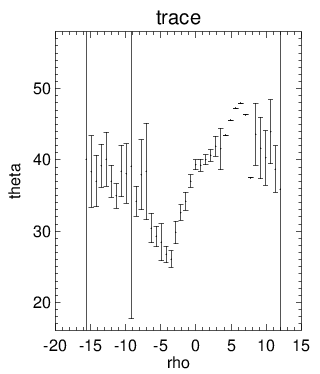
\includegraphics[width=0.23\textwidth]{Images/trace-plots/trace-plots-cpsbs/8143-3703.png}
    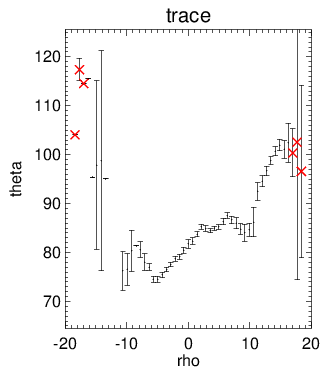
\includegraphics[width=0.23\textwidth]{Images/trace-plots/trace-plots-cpsbs/8313-6101.png}
    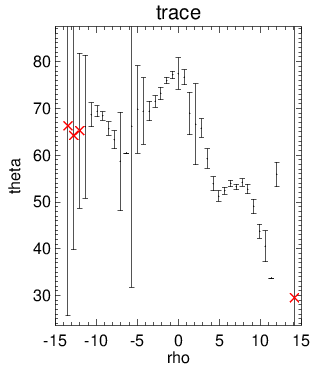
\includegraphics[width=0.23\textwidth]{Images/trace-plots/trace-plots-cpsbs/8315-3703.png}
    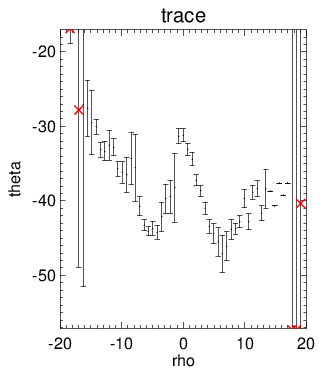
\includegraphics[width=0.23\textwidth]{Images/trace-plots/trace-plots-cpsbs/8331-6104.png}
    %
    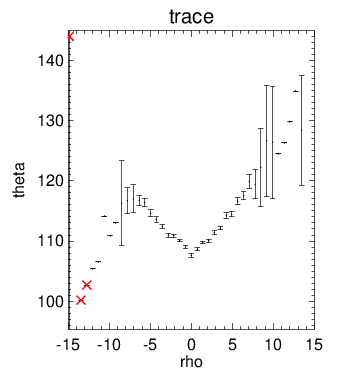
\includegraphics[width=0.23\textwidth]{Images/trace-plots/trace-plots-cpsbs/8555-3701.png}
    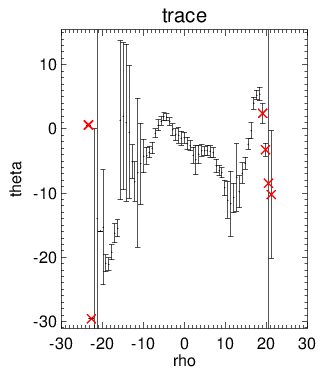
\includegraphics[width=0.23\textwidth]{Images/trace-plots/trace-plots-cpsbs/8623-9102.png}
    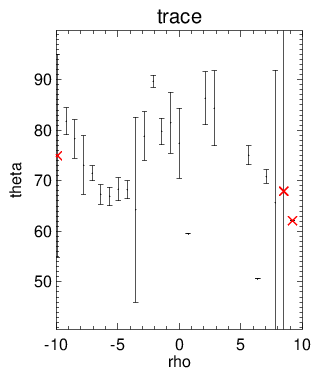
\includegraphics[width=0.23\textwidth]{Images/trace-plots/trace-plots-cpsbs/8655-1902.png}
    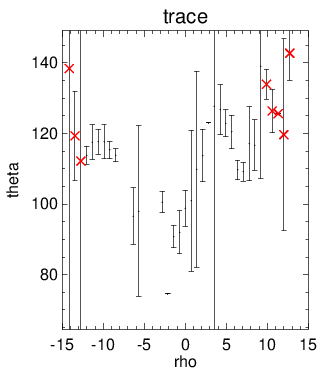
\includegraphics[width=0.23\textwidth]{Images/trace-plots/trace-plots-cpsbs/8713-3701.png}
    %
    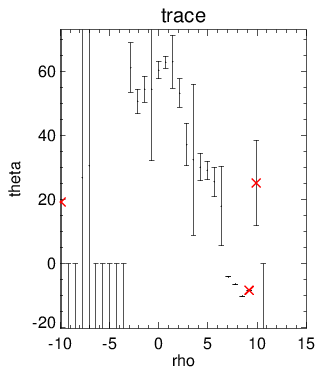
\includegraphics[width=0.23\textwidth]{Images/trace-plots/trace-plots-cpsbs/8725-1902.png}
    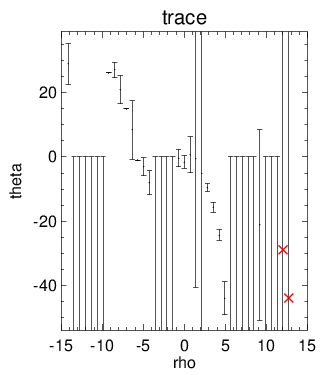
\includegraphics[width=0.23\textwidth]{Images/trace-plots/trace-plots-cpsbs/8933-3704.png}
    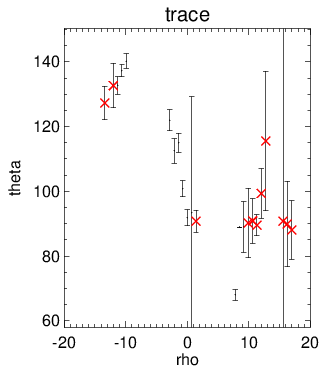
\includegraphics[width=0.23\textwidth]{Images/trace-plots/trace-plots-cpsbs/8934-9101.png}
    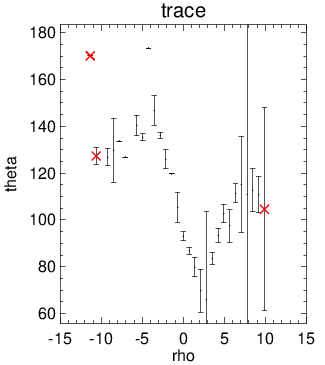
\includegraphics[width=0.23\textwidth]{Images/trace-plots/trace-plots-cpsbs/8935-12701.png}
    %
    \caption{Radon transform trace profiles of the stellar velocity fields of CPSB galaxies (set 1 of 2). The MaNGA plateifu identifiers are as follows, top row: 7964-1902, 8080-3702, 8081-3702, 8082-3704; second row: 8143-3703, 8313-6101, 8315-3703, 8331-6104; third row: 8555-3701, 8623-9102, 8655-1902, 8713-3701; bottom row: 8725-1902, 8933-3704, 8934-9101, 8935-12701.}
    \label{fig:Radon-traces-CPSBs-1}
\end{figure*}

\begin{figure*}
    \centering
    %
    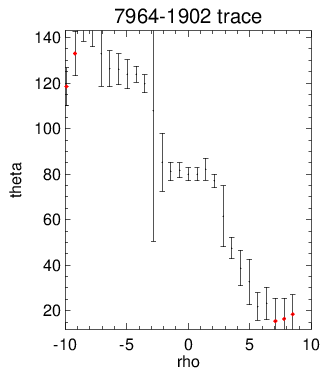
\includegraphics[width=0.24\textwidth]{Images/SN1-MC250/CPSBs/7694-1902-1-250.png}
    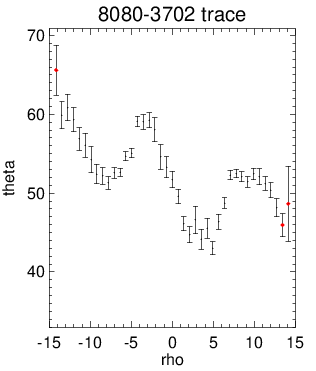
\includegraphics[width=0.24\textwidth]{Images/SN1-MC250/CPSBs/8080-3702-1-250.png}
    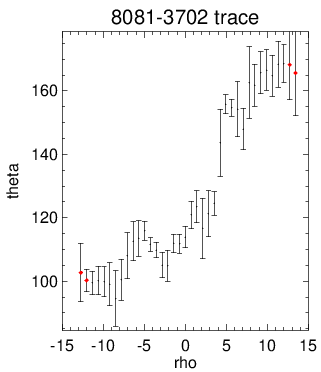
\includegraphics[width=0.24\textwidth]{Images/SN1-MC250/CPSBs/8081-3702-1-250.png}
    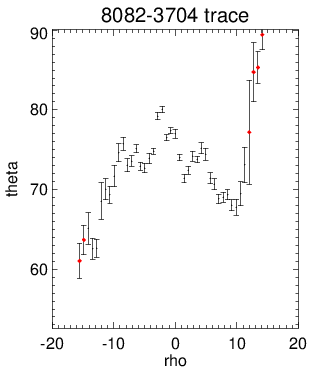
\includegraphics[width=0.24\textwidth]{Images/SN1-MC250/CPSBs/8082-3704-1-250.png}
    %
    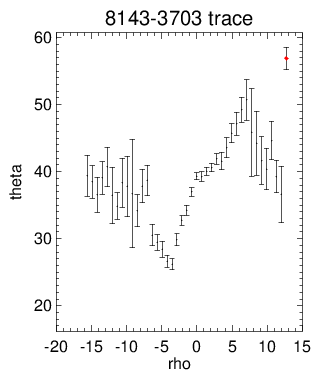
\includegraphics[width=0.24\textwidth]{Images/SN1-MC250/CPSBs/8143-3703-1-250.png}
    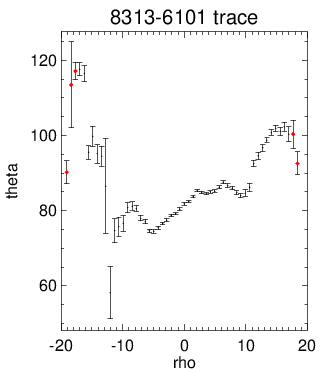
\includegraphics[width=0.24\textwidth]{Images/SN1-MC250/CPSBs/8313-6101-1-250.png}
    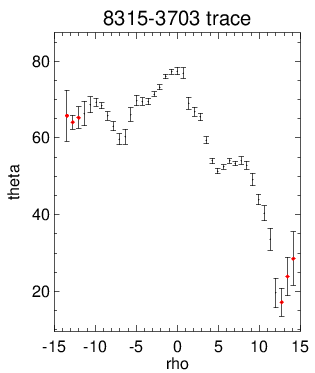
\includegraphics[width=0.24\textwidth]{Images/SN1-MC250/CPSBs/8315-3703-1-250.png}
    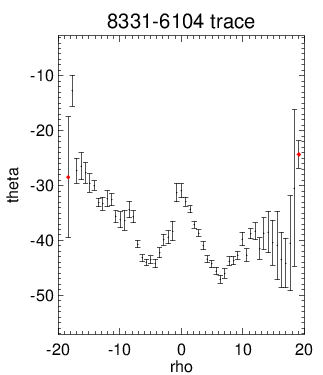
\includegraphics[width=0.24\textwidth]{Images/SN1-MC250/CPSBs/8331-6104-1-250.png}
    %
    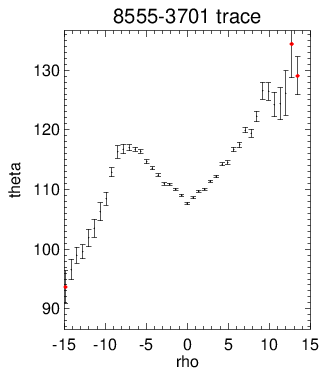
\includegraphics[width=0.24\textwidth]{Images/SN1-MC250/CPSBs/8555-3701-1-250.png}
    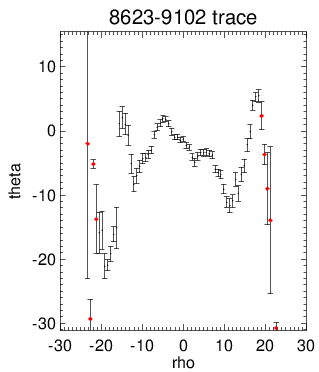
\includegraphics[width=0.24\textwidth]{Images/SN1-MC250/CPSBs/8623-9102-1-250.png}
    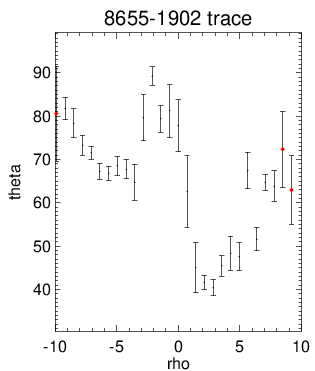
\includegraphics[width=0.24\textwidth]{Images/SN1-MC250/CPSBs/8655-1902-1-250.png}
    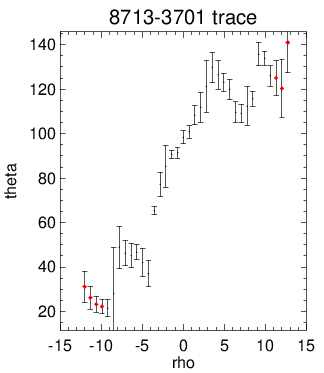
\includegraphics[width=0.24\textwidth]{Images/SN1-MC250/CPSBs/8713-3701-1-250.png}
    %
    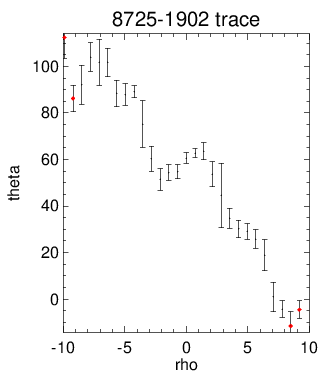
\includegraphics[width=0.23\textwidth]{Images/SN1-MC250/CPSBs/8725-1902-1-250.png}
    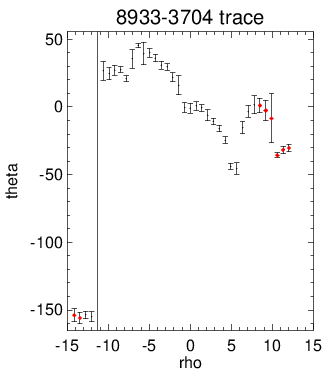
\includegraphics[width=0.23\textwidth]{Images/SN1-MC250/CPSBs/8933-3704-1-250.png}
    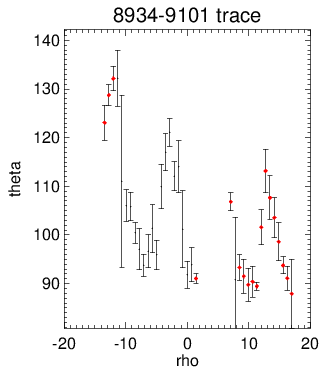
\includegraphics[width=0.23\textwidth]{Images/SN1-MC250/CPSBs/8934-9101-1-250.png}
    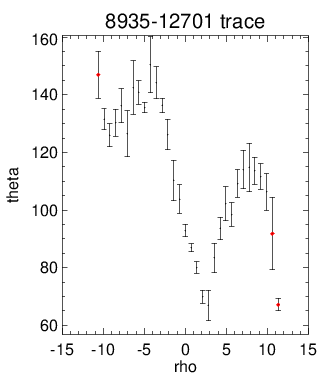
\includegraphics[width=0.23\textwidth]{Images/SN1-MC250/CPSBs/8935-12701-1-250.png}    
    %
    \caption{}
    \label{fig:Radon-traces-CPSBs-1-SN1-MC250}
\end{figure*}

\begin{figure*}
    \centering
    %
    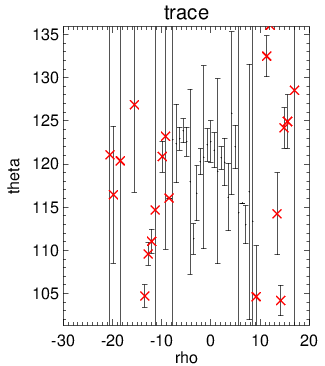
\includegraphics[width=0.23\textwidth]{Images/trace-plots/trace-plots-cpsbs/8938-6102.png}
    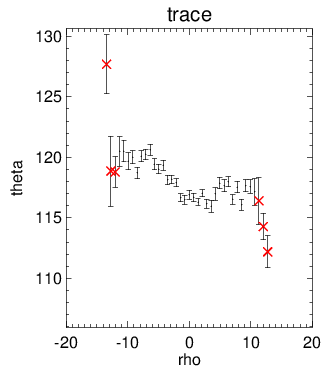
\includegraphics[width=0.23\textwidth]{Images/trace-plots/trace-plots-cpsbs/8941-3701.png}
    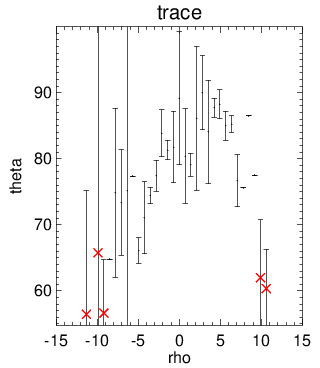
\includegraphics[width=0.23\textwidth]{Images/trace-plots/trace-plots-cpsbs/8944-1902.png}
    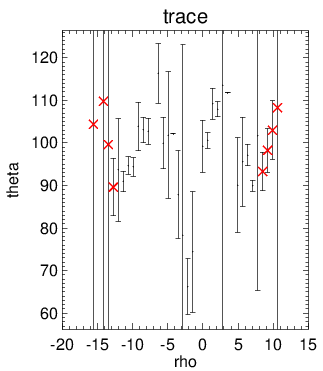
\includegraphics[width=0.23\textwidth]{Images/trace-plots/trace-plots-cpsbs/8950-3704.png}
    %
    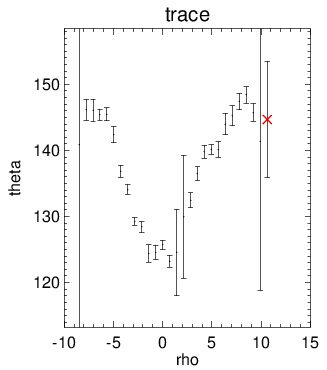
\includegraphics[width=0.23\textwidth]{Images/trace-plots/trace-plots-cpsbs/8979-1902.png}
    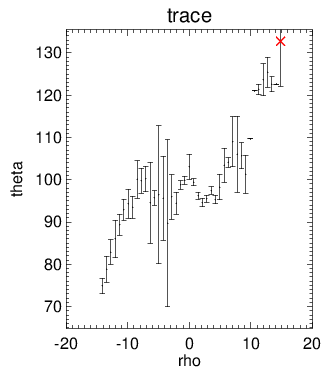
\includegraphics[width=0.23\textwidth]{Images/trace-plots/trace-plots-cpsbs/8996-3704.png}
    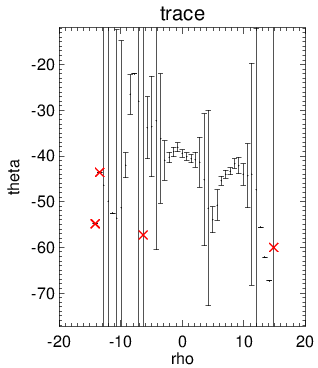
\includegraphics[width=0.23\textwidth]{Images/trace-plots/trace-plots-cpsbs/8997-3704.png}
    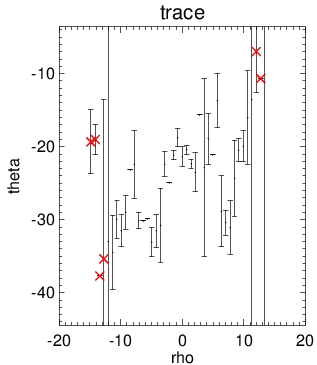
\includegraphics[width=0.23\textwidth]{Images/trace-plots/trace-plots-cpsbs/9047-3701.png}
    %
    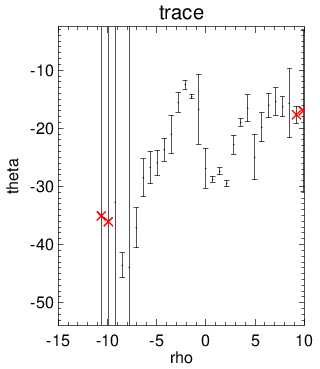
\includegraphics[width=0.23\textwidth]{Images/trace-plots/trace-plots-cpsbs/9085-1902.png}
    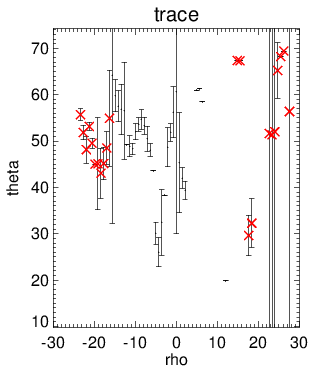
\includegraphics[width=0.23\textwidth]{Images/trace-plots/trace-plots-cpsbs/9493-12705.png}
    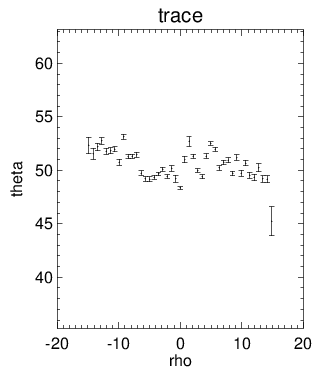
\includegraphics[width=0.23\textwidth]{Images/trace-plots/trace-plots-cpsbs/9494-3701.png}
    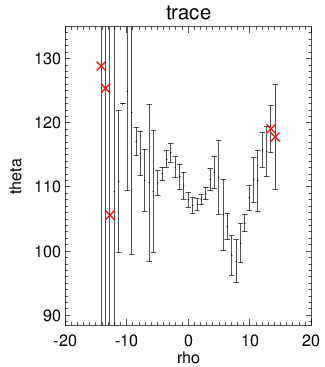
\includegraphics[width=0.23\textwidth]{Images/trace-plots/trace-plots-cpsbs/9494-3703.png}
    %
    \caption{Radon transform trace profiles of the stellar velocity fields of CPSB galaxies (set 2 of 2). The MaNGA plateifu identifiers are as follows, top row: 8938-6102, 8941-3701, 8944-1902, 8950-3704; second row: 8979-1902, 8996-3704, 8997-3704, 9047-3701; bottom row: 9085-1902, 9493-12705, 9494-3701, 9494-3703.}
    \label{fig:Radon-traces-CPSBs-2}
\end{figure*}

\begin{figure*}
    \centering
    %
    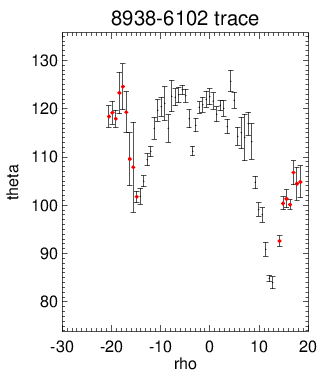
\includegraphics[width=0.23\textwidth]{Images/SN1-MC250/CPSBs/8938-6102-1-250.png}
    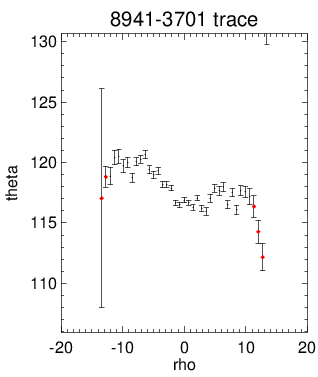
\includegraphics[width=0.23\textwidth]{Images/SN1-MC250/CPSBs/8941-3701-1-250.png}
    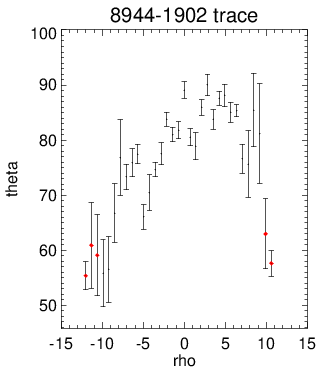
\includegraphics[width=0.23\textwidth]{Images/SN1-MC250/CPSBs/8944-1902-1-250.png}
    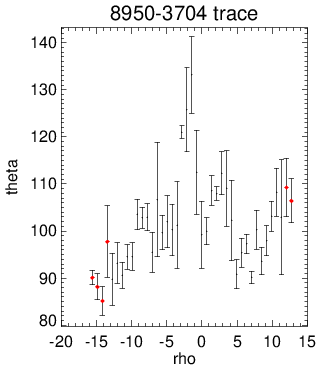
\includegraphics[width=0.23\textwidth]{Images/SN1-MC250/CPSBs/8950-3704-1-250.png}
    %
    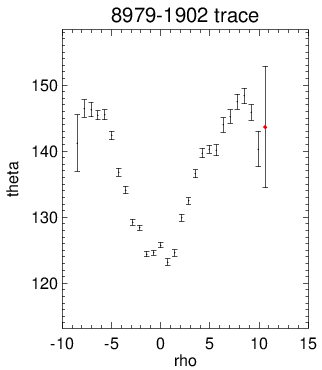
\includegraphics[width=0.23\textwidth]{Images/SN1-MC250/CPSBs/8979-1902-1-250.png}
    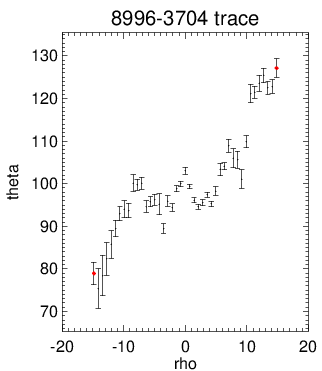
\includegraphics[width=0.23\textwidth]{Images/SN1-MC250/CPSBs/8996-3704-1-250.png}
    \includegraphics[width=0.23\textwidth]{Images/SN1-MC250/CPSBs/8997-3704-1-250.png}
    \includegraphics[width=0.23\textwidth]{Images/SN1-MC250/CPSBs/9047-3701-1-250.png}
    %
    \includegraphics[width=0.23\textwidth]{Images/SN1-MC250/CPSBs/9085-1902-1-250.png}
    \includegraphics[width=0.23\textwidth]{Images/SN1-MC250/CPSBs/9493-12705-1-250.png}
    \includegraphics[width=0.23\textwidth]{Images/SN1-MC250/CPSBs/9494-3701-1-250.png}
    \includegraphics[width=0.23\textwidth]{Images/SN1-MC250/CPSBs/9494-3703-1-250.png}
    %
    \caption{Radon transform trace profiles of the stellar velocity fields of CPSB galaxies (set 2 of 2). The Radon Trace plots were constructed with parameters SNCUT=1 and MC\_ITER=250. The MaNGA plateifu identifiers are as follows, top row: 8938-6102, 8941-3701, 8944-1902, 8950-3704; second row: 8979-1902, 8996-3704, 8997-3704, 9047-3701; bottom row: 9085-1902, 9493-12705, 9494-3701, 9494-3703.}
    \label{fig:Radon-traces-CPSBs-2-SN1-MC250}
\end{figure*}


\subsection{CPSB controls}
Radon transform trace profiles for the CPSB control galaxy sample group of are displayed in Figures \ref{fig:Radon-traces-CPSB-controls-1} and \ref{fig:Radon-traces-CPSB-controls-2}. Again, there is no significance in the split of CPSB Radon trace profiles between Figures \ref{fig:Radon-traces-CPSB-controls-1} and \ref{fig:Radon-traces-CPSB-controls-2}, other than to display these clearly on the page.

\begin{figure*}
    \centering
    \includegraphics[width=0.23\textwidth]{Images/trace-plots/trace-plots-cpsb-controls/8084-6103.png}    \includegraphics[width=0.23\textwidth]{Images/trace-plots/trace-plots-cpsb-controls/8262-3703.png}
    \includegraphics[width=0.23\textwidth]{Images/trace-plots/trace-plots-cpsb-controls/8262-12701.png}
    \includegraphics[width=0.23\textwidth]{Images/trace-plots/trace-plots-cpsb-controls/8335-12704.png}
    %
    \includegraphics[width=0.23\textwidth]{Images/trace-plots/trace-plots-cpsb-controls/8442-3704.png}
    \includegraphics[width=0.23\textwidth]{Images/trace-plots/trace-plots-cpsb-controls/8461-9102.png}
    \includegraphics[width=0.23\textwidth]{Images/trace-plots/trace-plots-cpsb-controls/8602-6101.png}
    \includegraphics[width=0.23\textwidth]{Images/trace-plots/trace-plots-cpsb-controls/8623-3702.png}
    %
    \includegraphics[width=0.23\textwidth]{Images/trace-plots/trace-plots-cpsb-controls/8624-12704.png}
    \includegraphics[width=0.23\textwidth]{Images/trace-plots/trace-plots-cpsb-controls/8625-3703.png}
    \includegraphics[width=0.23\textwidth]{Images/trace-plots/trace-plots-cpsb-controls/8716-12704.png}
    \includegraphics[width=0.23\textwidth]{Images/trace-plots/trace-plots-cpsb-controls/8727-12704.png}
    %
    \includegraphics[width=0.23\textwidth]{Images/trace-plots/trace-plots-cpsb-controls/8932-1901.png}
    \includegraphics[width=0.23\textwidth]{Images/trace-plots/trace-plots-cpsb-controls/8932-6103.png}
    \includegraphics[width=0.23\textwidth]{Images/trace-plots/trace-plots-cpsb-controls/8939-3701.png}
    \includegraphics[width=0.23\textwidth]{Images/trace-plots/trace-plots-cpsb-controls/8940-6101.png}
    %
    \caption{Radon transform trace profiles of the stellar velocity maps of CPSB control galaxies maps with RT input parameters SNCUT=1 and MC\_ITER=250 (set 1 of 2). The MaNGA plateifu identifiers are as follows, top row: 8084-6103, 8262-3703, 8262-12701, 8335-12704; second row: 8442-3704, 8461-9102, 8602-6101, 8623-3702; third row: 8624-12704, 8625-3703, 8716-12704, 8727-12704; bottom row: 8932-1901, 8932-6103, 8939-3701, 8940-6101.}
    \label{fig:Radon-traces-CPSB-controls-1}
\end{figure*}

\begin{figure*}
    \centering
    \includegraphics[width=0.23\textwidth]{Images/SN1-MC250/CPSB-CTRLs/8084-6103-1-250.png}
    \includegraphics[width=0.23\textwidth]{Images/SN1-MC250/CPSB-CTRLs/8262-3703-1-250.png}
    \includegraphics[width=0.23\textwidth]{Images/SN1-MC250/CPSB-CTRLs/8262-12701-1-250.png}
    \includegraphics[width=0.23\textwidth]{Images/SN1-MC250/CPSB-CTRLs/8335-12704-1-250.png}
    %
    \includegraphics[width=0.23\textwidth]{Images/SN1-MC250/CPSB-CTRLs/8442-3704-1-250.png}
    \includegraphics[width=0.23\textwidth]{Images/SN1-MC250/CPSB-CTRLs/8461-9102-1-250.png}
    \includegraphics[width=0.23\textwidth]{Images/SN1-MC250/CPSB-CTRLs/8602-6101-1-250.png}
    \includegraphics[width=0.23\textwidth]{Images/SN1-MC250/CPSB-CTRLs/8623-3702-1-250.png}
    %
    \includegraphics[width=0.23\textwidth]{Images/SN1-MC250/CPSB-CTRLs/8624-12704-1-250.png}
    \includegraphics[width=0.23\textwidth]{Images/SN1-MC250/CPSB-CTRLs/8625-3703-1-250.png}
    \includegraphics[width=0.23\textwidth]{Images/SN1-MC250/CPSB-CTRLs/8716-12704-1-250.png}
    \includegraphics[width=0.23\textwidth]{Images/SN1-MC250/CPSB-CTRLs/8727-12704-1-250.png}
    %
    \includegraphics[width=0.23\textwidth]{Images/SN1-MC250/CPSB-CTRLs/8932-1901-1-250.png}
    \includegraphics[width=0.23\textwidth]{Images/SN1-MC250/CPSB-CTRLs/8932-6103-1-250.png}
    \includegraphics[width=0.23\textwidth]{Images/SN1-MC250/CPSB-CTRLs/8939-3701-1-250.png}
    \includegraphics[width=0.23\textwidth]{Images/SN1-MC250/CPSB-CTRLs/8940-6101-1-250.png}
    %
    \caption{Radon transform trace profiles of the stellar velocity maps of CPSB control galaxies maps with RT input parameters SNCUT=1 and MC\_ITER=250 (set 1 of 2). The MaNGA plateifu identifiers are as follows, top row: 8084-6103, 8262-3703, 8262-12701, 8335-12704; second row: 8442-3704, 8461-9102, 8602-6101, 8623-3702; third row: 8624-12704, 8625-3703, 8716-12704, 8727-12704; bottom row: 8932-1901, 8932-6103, 8939-3701, 8940-6101.}
    \label{fig:Radon-traces-CPSB-controls-1-SN1-MC250}
\end{figure*}

\begin{figure*}
    \centering
    %
    \includegraphics[width=0.23\textwidth]{Images/trace-plots/trace-plots-cpsb-controls/8945-12703.png}
    \includegraphics[width=0.23\textwidth]{Images/trace-plots/trace-plots-cpsb-controls/8992-1902.png}
    \includegraphics[width=0.23\textwidth]{Images/trace-plots/trace-plots-cpsb-controls/8995-9101.png}
    \includegraphics[width=0.23\textwidth]{Images/trace-plots/trace-plots-cpsb-controls/9029-6103.png}
    %
    \includegraphics[width=0.23\textwidth]{Images/trace-plots/trace-plots-cpsb-controls/9043-6104.png}
    \includegraphics[width=0.23\textwidth]{Images/trace-plots/trace-plots-cpsb-controls/9048-6101.png}
    \includegraphics[width=0.23\textwidth]{Images/trace-plots/trace-plots-cpsb-controls/9505-12701.png}   
    \includegraphics[width=0.23\textwidth]{Images/trace-plots/trace-plots-cpsb-controls/9509-9101.png}
    %
    \includegraphics[width=0.23\textwidth]{Images/trace-plots/trace-plots-cpsb-controls/9870-12701.png}
    \includegraphics[width=0.23\textwidth]{Images/trace-plots/trace-plots-cpsb-controls/9871-1901.png}    
    \includegraphics[width=0.23\textwidth]{Images/trace-plots/trace-plots-cpsb-controls/9876-3701.png}
    %
    \caption{Radon transform trace profiles of the stellar velocity maps of CPSB control galaxies with RT input parameters SNCUT=3 and MC\_ITER=1 (set 2 of 2). The MaNGA plateifu identifiers are as follows, top row: 8945-12703, 8992-1902, 8995-9101, 9029-6103; second row: 9043-6104, 9048-6101, 9505-12701, 9509-9101; bottom row: 9870-12701, 9871-1901, 9876-3701.}
    \label{fig:Radon-traces-CPSB-controls-2}
\end{figure*}

\begin{figure*}
    \centering
    %
    \includegraphics[width=0.23\textwidth]{Images/SN1-MC250/CPSB-CTRLs/8945-12703-1-250.png}
    \includegraphics[width=0.23\textwidth]{Images/SN1-MC250/CPSB-CTRLs/8992-1902-1-250.png}
    \includegraphics[width=0.23\textwidth]{Images/SN1-MC250/CPSB-CTRLs/8995-9101-1-250.png}
    \includegraphics[width=0.23\textwidth]{Images/SN1-MC250/CPSB-CTRLs/9029-6103-1-250.png}
    %
    \includegraphics[width=0.23\textwidth]{Images/SN1-MC250/CPSB-CTRLs/9043-6104-1-250.png}
    \includegraphics[width=0.23\textwidth]{Images/SN1-MC250/CPSB-CTRLs/9048-6101-1-250.png}
    \includegraphics[width=0.23\textwidth]{Images/SN1-MC250/CPSB-CTRLs/9505-12701-1-250.png}   
    \includegraphics[width=0.23\textwidth]{Images/SN1-MC250/CPSB-CTRLs/9509-9101-1-250.png}
    %
    \includegraphics[width=0.23\textwidth]{Images/SN1-MC250/CPSB-CTRLs/9870-12701-1-250.png}
    \includegraphics[width=0.23\textwidth]{Images/SN1-MC250/CPSB-CTRLs/9871-1901-1-250.png}    
    \includegraphics[width=0.23\textwidth]{Images/SN1-MC250/CPSB-CTRLs/9876-3701-1-250.png}
    %
    \caption{Radon transform trace profiles of the stellar velocity maps of CPSB control galaxies with RT input parameters SNCUT=3 and MC\_ITER=1 (set 2 of 2). The MaNGA plateifu identifiers are as follows, top row: 8945-12703, 8992-1902, 8995-9101, 9029-6103; second row: 9043-6104, 9048-6101, 9505-12701, 9509-9101; bottom row: 9870-12701, 9871-1901, 9876-3701.}
    \label{fig:Radon-traces-CPSB-controls-2-SN1-MC250}
\end{figure*}

\section{Analysis}
\label{sec:analysis}

To follow.

\section{Conclusions}
\label{sec:conclusions}

To follow.



%%%%%%%%%%%%%%%%%%%%%%%%%%%%%%%%%%%%%%%%%%%%%%%%%%

%%%%%%%%%%%%%%%%%%%% REFERENCES %%%%%%%%%%%%%%%%%%

% The best way to enter references is to use BibTeX:

\bibliographystyle{mnras}
\bibliography{JPbib2019} % if your bibtex file is called example.bib

%%%%%%%%%%%%%%%%%%%%%%%%%%%%%%%%%%%%%%%%%%%%%%%%%%

%%%%%%%%%%%%%%%%% APPENDICES %%%%%%%%%%%%%%%%%%%%%

% \appendix
%
% \section{Some extra material}

% If you want to present additional material which would interrupt the flow of the main paper,
% it can be placed in an Appendix which appears after the list of references.

%%%%%%%%%%%%%%%%%%%%%%%%%%%%%%%%%%%%%%%%%%%%%%%%%%


% Don't change these lines
\bsp	% typesetting comment
\label{lastpage}
\end{document}

% End of mnras_template.tex